\section{The COReX feature extractor}

\begin{figure}
  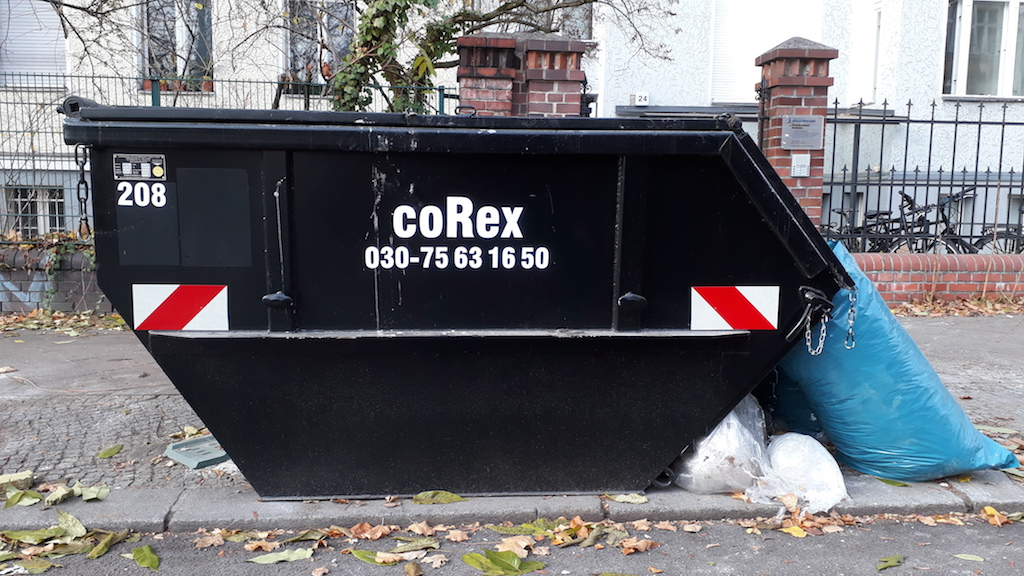
\includegraphics[scale=.3]{corexcontainer.jpg}
  \caption{The COReX feature extractor}  
\end{figure}



COReX is a piece of software designed to extract a large number of normalised feature counts\footnote{Currently, COReX extracts over 60 features. The complete list is provided in the appendix.} at the document level from German text. Most features correspond to linguistic concepts (such as occurrences of a particular parts-of-speech, periphrastic passive and perfect constructions, non-standard morphological forms), alongside a few features which are not strictly linguistic (such as type/token ratio and word/sentence lengths). 
COReX does not perform linguistic annotation by itself, but rather relies on linguistic pre-processing, typically performed automatically by dedicated annotation tools.
COReX is implemented in Python and is easily extendable to include additional features (which, in most cases, will require additional pre-processing of the input corpus).\footnote{Another note.}
%The input format is vertical text (one token per line) with token level annotations in columns 2 through n, and token spans represented as XML-elements (this corresponds to the input format required by tools such as OpenCWB and NoSketchEngine).
%Required XML-elements are doc (document) and s (sentence).

In order to extract the full range of features, the data must include part-of-speech tags (STTS; \citealp{Schiller-ea1999}), morphological features (such as those produced by MarMoT; \citealp{MuellerSchmidSchuetze2013}), named entity annotations (such as those produced by the Stanford NER tagger; \citealp{FinkelGrenagerManning2005}) as well as topological field annotations (as produced by the Berkeley parser; \cite{PetrovKlein2007}, \cite{CheungPenn2009}, \cite{Telljohann-ea2012}).

%For some annotation layers, such as morphological features and topological fields, a particular formatting is required.
%COReX outputs a modified version of the input data where normalised document-level feature counts are added as attribute-value pairs to the opening <doc > tag for each document.
%Moreover, a number of non-normalised counts (such as perfect and passive) are added as attribute-value pairs to the <s > tag for each sentence. Features include non-linguistic categories such as mean word length and mean sentence length; counts for individual parts-of-speech; ...
 
%COReX outputs a modified version of the input data where normalised document-level feature counts are added as attribute-value pairs to the opening <doc > tag for each document.
%Moreover, a number of non-normalised counts (such as perfect and passive) are added as attribute-value pairs to the <s > tag for each sentence. Features include non-linguistic categories such as mean word length and mean sentence length; counts for individual parts-of-speech; ...




[Distribution of features in COW data; clustering]
